\chapter{Diseño de la variante \emph{DC-Net}}\label{cap3}

\section{Conceptos Básicos}

\begin{itemize}
    \item Participante: agente que participa activamente del protocolo, ya sea 
    enviando un mensaje o contribuyendo para aumentar el tamaño del 
    \emph{anonimity-set} y así ocultar ``de mejor manera'' a los emisores de 
    mensajes. 
    \item Ronda: serie de pasos (descritos a partir de la próxima sección) que 
    se llevan a cabo (principalmente intercambiando mensajes entre los 
    participantes) con el objetivo de ir reduciendo, ronda a ronda, los mensajes 
    enviados por cada participante.  
    \item Mensaje: información que cada participante desea transmitir de 
    manera anónima. Generalmente se relacionará a un conjunto de caracteres 
    (representados como \emph{String}), en un cierto idioma, que se desea 
    comunicar.
    \item Sesión: conjunto de rondas que se necesitan realizar para que pueda 
    ser transmitido, a lo más, un mensaje por participante. Al principio de 
    cada sesión se le brinda la oportunidad a cada participante de decidir si 
    enviará o no un mensaje. Luego que cada participante realizó su decisión, 
    se inicia el protocolo descrito a continuación, que tiene como objetivo 
    que cada uno de los mensajes que se decidieron enviar, se envíen de manera 
    anónima al resto de los participantes.
    \item Sala: conjunto de participantes corriendo una sesión del protocolo.
    \item Observador Externo: cualquier agente (a excepción de los propios 
    participantes) que pueda estar monitoreando, tanto los mensajes 
    resultantes del protocolo, como mensajes intermedios intercambiados entre 
    los distintos participantes durante la realización del protocolo. A no ser 
    que se explicite, todos los mensajes del protocolo pueden ser monitoreados 
    por un observador externo y se consideran públicos.
    \item Adversario: agente que tiene como finalidad, ya sea encontrar al 
    emisor de un cierto mensaje, o bien, alterar el comportamiento ``normal'' 
    del protocolo (retrasándolo o impidiendo su total realización). Este 
    adversario puede ser un mismo participante del protocolo (al cual 
    llamaremos participante malicioso) o un observador externo.
    \item Canal de comunicación: enlace existente entre dos nodos del 
    sistema. Estos canales deben ser autenticados y no encriptados, es decir, todos los mensajes 
    enviados en el protocolos deben ir firmados utilizando un protocolo 
    de clave pública y éstos pueden enviarse ``en plano'', de manera que cualquier 
    monitoreo tiene la capacidad de observar los mensajes enviados, pero no 
    incorporar mensajes al sistema por parte de emisores no participantes del 
    protocolo.
\end{itemize}

\section{Resolución de Colisiones}

El protocolo propuesto tiene como principal característica el no evitar las 
posibles colisiones que puedan producirse (en contraposición con otros 
protocolos que se enfocan en evitar la colisión de mensajes). De producirse la 
colisión, se debe resolver corriendo nuevas rondas del protocolo, pero 
solamente permitiendo que un subconjunto de los mensajes colisionados puedan 
re-enviarse en cada una de las rondas subsecuentes, produciendo así que en 
cada nueva ronda que se desarrolle, exista un menor número de mensajes 
colisionando, resultando así en rondas que se desarrollen sin colisión, 
enviándose los mensajes de manera solitaria, lo que les permite ser legibles 
por el resto de los participantes. Esta técnica de resolución de colisiones es 
conocida como \emph{superposed receiving} \cite{franck2014dining}.

Las rondas que se desarrollan durante el protocolo son de dos tipos: reales y 
virtuales. En las rondas reales es necesario el envío de múltiples mensajes 
por parte de los participantes, involucrando el uso de varias herramientas 
criptográficas con el objetivo de evitar que participantes maliciosos alteren 
el normal desarrollo del protocolo. En cambio las rondas virtuales son tales 
que su resultado puede inferirse por rondas reales ejecutadas anteriormente, 
por lo que no es necesario el envío de ningún mensaje por parte de los 
participantes (las rondas reales cuestan trabajo por parte de los 
participantes, y las rondas virtuales no). Si la primera colisión de mensajes 
es de $n$ mensajes, eso implica que es necesario ejecutar $n$ rondas reales 
para poder resolver dicha colisión. Esta técnica es conocida como 
\emph{inference cancellation} \cite{yu2005sicta}.

En la Figura \ref{fig:supreceiving_tree-1} se muestra un ejemplo de resolución 
de colisiones, mostrando a grandes rasgos la idea mencionada de no evitar las 
colisiones sino resolverlas de manera eficiente. En este ejemplo, 5 mensajes 
colisionan en la primera ronda, lo que significa que en las rondas 
subsecuentes (segunda y tercera), un subconjunto de esos 5 mensajes son 
reenviados (una parte de ellos se reenvía en la segunda ronda, y el resto se 
reenvía en la tercera ronda). Importante notar que el criterio para decidir si 
un mensaje es reenviado en la ronda 2 o en la ronda 3, tiene relación con el 
promedio de los mensajes que colisionaron (esta idea es explicada con mayor 
detalle más adelante). Si en las rondas 2 ó 3 se vuelve a producir una 
colisión (que es el caso que se produce en el ejemplo), se vuelve a realizar 
la misma idea, es decir, un subconjunto de los mensajes se reenvían en las 
rondas subsecuentes (para la colisión de la ronda 2, los mensajes se reenvían 
en las rondas 4 y 5; para la colisión de la ronda 3, los mensajes se reenvían 
en las rondas 6 y 7). Como regla general, si la colisión se produce en la 
ronda $k$, los mensajes se reenvían en las rondas $2k$ y $2k + 1$. Este 
protocolo de resolución se realiza hasta que todos los mensajes que 
colisionaron en la ronda 1, son reenviados en rondas de forma individual, es 
decir, no colisionaron con ningún otro mensaje (en el ejemplo, esto se produce 
en las rondas 4, 5, 6, 14 y 15). Por último debemos mencionar las rondas 
virtuales que se ejecutan. En la Figura se puede observar que la ronda 3 es 
virtual, ya que su valor puede ser derivado a partir de los valores que se 
obtuvieron en las rondas 1 y 2. De manera general, las rondas virtuales poseen 
la forma $2k + 1$, cuyo valor puede ser derivado a partir de los valores 
generados en las rondas $k$ y $2k$ (en la Figura 
\ref{fig:supreceiving_tree-1}, las rondas virtuales están 
expresadas a partir de líneas punteadas alrededor de los mensajes que son 
enviados).

 \begin{figure}[H]
 \begin{centering}
 \footnotesize
 \pgfdeclarelayer{background layer}
 \pgfdeclarelayer{foreground layer}
 \pgfsetlayers{background layer,main,foreground layer}
 \begin{tikzpicture}[yscale=0.8]
 \begin{scope}[level distance=2.0cm,
 sibling distance=4cm,level/.style={sibling distance=3.8cm/#1},
 edge from parent/.style={draw,very thick},
 block/.style ={rectangle, draw=black, thick, text centered,  inner sep=0.12cm,font=\footnotesize},
 blockx/.style ={rectangle, dashed, draw=black, very thick, text centered,  inner sep=0.12cm,font=\footnotesize}]
 \begin{pgfonlayer}{foreground layer}
 \node[block] (n1){$\underbrace{M_1+M_2+M_3+M_4+M_5}_{\displaystyle (5,130)}$}
 % [edge from parent fork down]
 child {node (n21)[block] {$\underbrace{M_2+M_4}_{\displaystyle (2,28)}$} 
 child {node (n2x)[block,yshift=-1.6cm] {$\underbrace{M_2}_{\displaystyle (1,11)}$} edge from parent node[fill=white,anchor=east,xshift=-0.05cm] {$<14 $}}
 child {node (n2a)[blockx,yshift=-3.2cm] {$\underbrace{M_4}_{\displaystyle (1,17)}$}}
 edge from parent node[fill=white,anchor=east,xshift=-0.25cm] {$<26$}}
 child {node (n22)[blockx,yshift=-1.6cm] {$\underbrace{M_1+M_3+M_5}_{\displaystyle (3,102)}$}
 child {node (n31)[block,yshift=-3.2cm] {$\underbrace{M_3}_{\displaystyle (1,28)}$}edge from parent node[fill=white,anchor=east,xshift=-0.05cm] {$<34 $~}}
 child {node (n32)[blockx,yshift=-4.8cm] {$\underbrace{M_1+M_5}_{\displaystyle (2,74)}$}
 child {node (n3f)[block] {$\underbrace{M_1}_{\displaystyle (1,36)}$}edge from parent node[fill=white,anchor=east,xshift=-0.1cm] {$<37 $~}}
 child {node (n3g)[blockx,yshift=-1.6cm] {$\underbrace{M_5}_{\displaystyle (1,38)}$}}}
 };
 \end{pgfonlayer}

 %\node[anchor=east] at (n1.west){400 $\sim$};
 %\node[anchor=east] at (n21.west){410 $\sim$};
 %\node[anchor=west] at (n22.east){$\sim$ 420};

 %\draw (n1.north) node [anchor=south] {1};
 %\draw (n21.north) node [anchor=south] {2};
 %\draw (n2x.north) node [anchor=south] {3};

 \path []($(n1)+ (-5.0cm,1.0cm)$) -- node[above]{$R^{(k)}$} +(10cm,0);

 \begin{pgfonlayer}{background layer}
 \draw [densely dotted]($(n1)+ (-5.0cm,1cm)$) node [above,xshift=0.8cm]{round id $k$}-- +(12.1cm,0);
 \draw [densely dotted]($(n1)+ (-5.0cm,-1cm)$) node [above,xshift=0.8cm]{$1$}-- +(12.1cm,0) node[above,anchor=south west,xshift=-2.5cm]{$R^{(1)}=\sum^n_{i=1}O^{(1)}_i$};
 \draw [densely dotted]($(n1)+ (-5.0cm,-3cm)$) node [above,xshift=0.8cm]{$2$}-- +(12.1cm,0) node[above,anchor=south west,xshift=-2.5cm]{$R^{(2)}=\sum^n_{i=1}O^{(2)}_i$};
 \draw [densely dotted]($(n1)+ (-5.0cm,-5cm)$) node [above,xshift=0.8cm]{$3$}-- +(12.1cm,0) node[above,anchor=south west,xshift=-2.5cm]{$R^{(3)}=R^{(1)}-R^{(2)}$};
 \draw [densely dotted]($(n1)+ (-5.0cm,-7cm)$) node [above,xshift=0.8cm]{$4$}-- +(12.1cm,0) node[above,anchor=south west,xshift=-2.5cm]{$R^{(4)}=\sum^n_{i=1}O^{(4)}_i$};
 \draw [densely dotted]($(n1)+ (-5.0cm,-9cm)$) node [above,xshift=0.8cm]{$5$}-- +(12.1cm,0) node[above,anchor=south west,xshift=-2.5cm]{$R^{(5)}=R^{(2)}-R^{(4)}$};
 \draw [densely dotted]($(n1)+ (-5.0cm,-11cm)$) node [above,xshift=0.8cm]{$6$}-- +(12.1cm,0) node[above,anchor=south west,xshift=-2.5cm]{$R^{(6)}=\sum^n_{i=1}O^{(6)}_i$};
 \draw [densely dotted]($(n1)+ (-5.0cm,-13cm)$) node [above,xshift=0.8cm]{$7$}-- +(12.1cm,0) node[above,anchor=south west,xshift=-2.5cm]{$R^{(7)}=R^{(3)}-R^{(6)}$};
 \draw [densely dotted]($(n1)+ (-5.0cm,-15cm)$) node [above,xshift=0.8cm]{$14$}-- +(12.1cm,0) node[above,anchor=south west,xshift=-2.5cm]{$R^{(14)}=\sum^n_{i=1}O^{(14)}_i$};
 \draw [densely dotted]($(n1)+ (-5.0cm,-17cm)$) node [above,xshift=0.8cm]{$15$}-- +(12.1cm,0) node[above,anchor=south west,xshift=-2.5cm]{$R^{(15)}=R^{(7)}-R^{(14)}$};
 \end{pgfonlayer}

 \node[inner sep=0cm,fit=(n1) (n3g) (n2x)] (la) {};
 %\node at (la.south)[below=0.3cm,inner sep=0,font=\small] {(a) Collision resolution tree.};
 \end{scope}


 \end{tikzpicture}
 \par\end{centering}

 \protect\caption{Ejemplo de árbol de resolución de colisiones utilizando 
 \emph{superposed receiving}.}
 \label{fig:supreceiving_tree-1}
 \end{figure}

\section{Compartición de Claves}

Una ronda real comienza con el proceso de compartición de claves entre cada 
par de participantes presentes en la sala. Este proceso debe realizarse, 
tomando un cuenta un posible adversario que esté monitoreando el canal de 
comunicación existente entre dos participantes cualquiera.

Para solucionar este problema se propone el uso del algoritmo 
\emph{Diffie-Hellman} \cite{diffie1976new}, el cual permite generar un valor 
secreto compartido entre dos agentes, cuyo canal de comunicación es 
monitoreado por un adversario.

Luego que cada par de participantes $\{P_i, P_j\}$ ejecuten el algoritmo 
\emph{Diffie-Hellman}, obtendrán un valor secreto $k_{ij}$ 
(y se define que $k_{ij} = -k_{ji}$). Para futuros pasos del protocolo, es 
necesario que ejecuten este proceso dos veces, ya que es necesario que cuenten 
con un segundo valor compartido $r(k_{ij})$ (también se define que 
$r(k_{ij}) = -r(k_{ji})$).

Si bien el proceso descrito (acuerdo \emph{Diffie-Hellman}) no alcanza 
seguridad incodicional (como sí lo hace el resto del protocolo \emph{DC-Net}), 
es posible alcanzarla precalculando estas claves en forma \emph{offline} vía 
un canal privado. Por simplificación, la implementación realizada para este 
trabajo utiliza \emph{Diffie-Hellman}.

\subsection{\emph{Commitments} sobre las claves}

Posteriormente cada participante $P_i$ debe realizar un \emph{commitment} a 
cada valor $k_{ij}$ que posee compartido con cada otro participante $P_j$, 
utilizando como aleatoriedad el segundo valor compartido $r(k_{ij})$. Así cada 
participante $P_i$ calcula $n - 1$ de los siguientes valores 
$c_{k_{ij}} = g^{k_{ij}} h^{r(k_{ij})}$.

Luego de esto, cada participante $P_i$ genera dos valores. El primero es 
la suma de todas las claves compartidas que posee $K_i = \sum k_{ij}$. El 
segundo valor es un \emph{commitment} sobre dicho valor, calculado utilizando 
los valores $c_{k_{ij}}$, esto es, 
$c_{K_i} = \prod c_{k_{ij}}$.

Finalmente cada participante $P_i$ enviará al resto de la sala vía 
\emph{broadcast} su \emph{commitment} $c_{K_i}$ junto con una 
\emph{zero-knowledge proof} demostrando que conoce los valores ``escondidos'' 
dentro del \emph{commitment} $c_{K_i}$.

\subsection{Verificación de los valores enviados}

Cada participante, al recibir los \emph{commitments} enviados por el resto de 
la sala, debe verificar que se cumple la siguiente propiedad: 
$\prod c_{K_i} = 1$ (esto se debe a la cancelación que se debe producir al 
sumar las claves). Si es que lo anterior no se produce, es resultado de que 
uno (o varios) de los participantes envió un valor incorrecto dentro de su 
\emph{commitment} respectivo, lo que implicaría una no cancelación de las 
claves compartidas en etapas subsecuentes del protocolo, alterando la entrega 
de los mensajes.

Es posible encontrar al(a los) participante(s) culpable(s) de enviar 
información errónea. Para ello cada participante $P_j$ revelará cada valor 
$c_{k_{ji}}$ calculado anteriormente. Luego de esto, el resto de la sala puede 
verificar que se deben cumplir dos propiedades: 
(1) $c_{K_j} = \prod c_{k_{ji}}$, que se debe tener por definición, y 
(2) $c_{k_{ij}} c_{k_{ji}} = 1$, lo cual se debe a la cancelación de las 
claves compartidas. Si alguna de las dos propiedades anteriores no se cumplen, 
el participante $P_j$ es malicioso y deben tomarse las medidas pertinentes que 
considere la sala, como por ejemplo, expulsión de los participantes maliciosos.

\section{Formato del Mensaje}

Al principio de una sesión, cada participante $P_i$ debe decidir si desea 
comunicar un mensaje $msg$ al resto de la sala o no. De querer enviar un 
mensaje, habrán rondas que deberá enviar $m_i = msg$, y otras que enviará 
$m_i = 0$. De no querer transmitir un mensaje, en todas las rondas enviará 
$m_i = 0$. 

Para que el protocolo funcione correctamente, es necesario que dicho mensaje 
$m_i$ se concatene con otros valores, permitiendo el correcto manejo de 
colisiones de mensajes (lo cual es explicado más adelante en el documento). 
Estos valores auxiliares son los siguientes:
\begin{itemize}
    \item $b_i$: bit que indica si el participante está, en la presente ronda, 
    enviando un mensaje distinto a cero o no ($b_i = 1 ssi m_i \neq 0$).
    \item $pad_i$: cadena de bits aleatoria que se añade para prevenir 
    colisión de mensajes iguales, que podría desembocar en que la sesión nunca 
    finalice.
\end{itemize}

Con estos valores establecidos, en cada ronda, cada participante $P_i$ debe 
formar el valor $M_i$ descrito en las figuras \ref{fig:M_sending} y 
\ref{fig:M_not_sending}. En dichas figuras se muestra el formato cuando 
el participante envía $m_i \neq 0$, y cuando el participante envía 
$m_i = 0$ (que significa $M_i = 0$).

\begin{figure}[H]
  \centering
    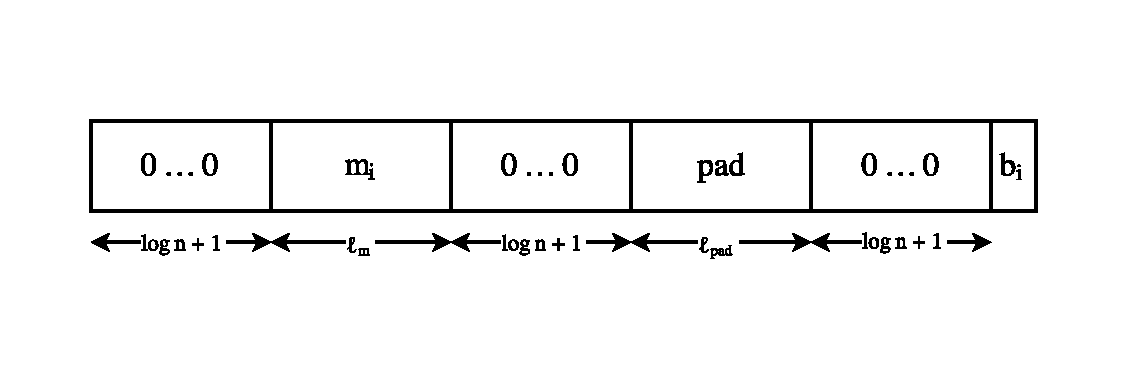
\includegraphics[width=1\textwidth]{imagenes/message-format(1).pdf}
  \caption{Formato de $M_i$ cuando se envía un mensaje}
  \label{fig:M_sending}
\end{figure}

\begin{figure}[H]
  \centering
    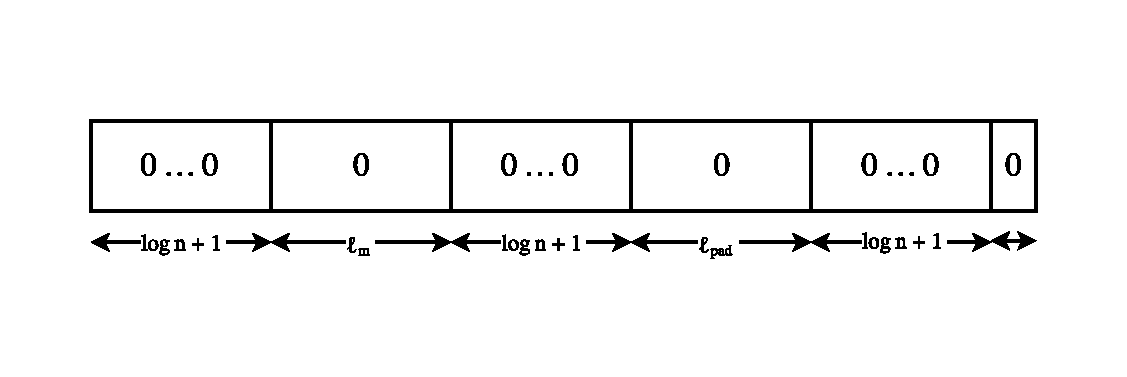
\includegraphics[width=1\textwidth]{imagenes/message-format-nomessage.pdf}
  \caption{Formato de $M_i$ cuando no se envía un mensaje}
  \label{fig:M_not_sending}
\end{figure}

Las cadenas de bits compuestas por 0s puestas entremedio de los valores, 
sirven para prevenir \emph{overflows} de los valores, impidiendo que se altere 
el resultado final al ocurrir una colisión.

\section{Correctitud del Formato del Mensaje}

Para que el protocolo tenga un correcto funcionamiento en el manejo de 
colisiones, es imperioso que el formato del mensaje $M_i$ se respete por todos 
los participantes. Para ello se debe satisfacer una de las siguientes 
restricciones:
\begin{itemize}
    \item Si $b_i = 0$, entonces $m_i = 0$
    \item $b_i = 1$
\end{itemize}

En la primera alternativa, se le fuerza al participante a que si esta diciendo 
que no envía un mensaje ($b_i = 0$), no lo envíe ($m_i = 0$). En la segunda 
opción, se le permite cualquier valor de $m_i$ siempre y cuando se cumpla que 
$b_i = 1$.

\subsection{\emph{Commitments} sobre los valores individuales}

Para poder demostrar que el mensaje $M_i$ posee un correcto formato, cada 
participante $P_i$  debe primero realizar \emph{commitments} a cada uno de los 
valores $\{m_i, pad_i, b_i\}$. Para ello, se escogen valores aleatorios 
$\{r(m_i), r({pad}_i), r(b_i)\}$ y se calculan los valores 
$c_{m_i} = g^{m_i} h^{r(m_i)}; c_{pad_i} = g^{pad_i} h^{r({pad}_i)}; 
c_{b_i} = g^{b_i} h^{r(b_i)}$ (\emph{commitments} a los valores individuales 
anteriormente descritos).

\subsection{\emph{Zero-knowledge Proof} sobre formato del mensaje}

Ahora es momento que cada participante genere una \emph{zero-knowledge proof} 
que demuestre que el mensaje $M_i$ esta bien formado. Para ello es necesario 
establecer primero si en la presente ronda el participante enviará un mensaje 
($m_i \neq 0$) o no ($m_i = 0$).

\begin{enumerate}
    \item Si el participante i-ésimo no envía un mensaje ($m_i = 0$): para 
    demostrar que el formato es correcto cuando no se necesita enviar un 
    mensaje, cada participante debe demostrar la primera restricción que se 
    mostró anteriormente, esto es, que $b_i = 0 \land m_i = 0$.
    
    Es importante notar que cuando sucede lo anterior, los valores de los 
    \emph{commitments} anteriormente descritos quedan de la siguiente manera: 
    $c_{m_i} = h^{r(m_i)}; c_{b_i} = h^{r(b_i)}$.
    
    Para ello, usando \emph{ZKPs}, el participante debe demostrar que conoce 
    los valores $\{r(m_i), r(b_i)\}$ contenidos en dichos \emph{commitments}.
    
    \item Envío de mensaje ($m_i \neq 0$): para demostrar que el formato es 
    correcto cuando necesita enviar un mensaje, debe demostrar la segunda 
    restricción, esto es solamente que $b_i = 1$.
    
    Al igual que en el caso anterior el \emph{commitment} asociado queda con 
    un formato particular $c_{b_i} = g h^{r(b_i)}$.
    
    En este caso se le va a pedir al participante demostrar que conoce el 
    logaritmo discreto $r(b_i)$ de $g^{-1} c_{b_i} = h^{r(b_i)}$ en base $h$.
\end{enumerate}

Como no se puede saber si el participante enviará o no un mensaje 
(comprometería su anonimato) se va a solicitar que demuestre cualquiera de las 
dos condiciones anteriores. La \emph{zero-knowledge proof-of-knowledge} (no 
interactiva) que necesita demostrar cada participante es la siguiente: 
$$\mathtt{PoK_i^{format}} = PoK\{(r(m_i), r(b_i)) : (c_{m_i} = h^{r(m_i)} 
\land c_{b_i} = h^{r(b_i)}) \lor (g^{-1} c_{b_i} = h^{r(b_i)})\}$$

\subsection{Envío de valores a la sala}

Después de todos los cálculos anteriores, cada participante $P_i$ debe enviar 
al resto de la sala vía \emph{broadcast} los siguientes valores: 
$\{c_{m_i}, c_{pad_i}, c_{b_i}, \mathtt{PoK_i^{format}}\}$ (los tres 
\emph{commitments} calculados y la demostración correspondiente).

\subsection{Verificación de la demostración}

Después de que toda la sala haya recibido todos los conjuntos de valores 
enviados por cada uno de los participantes, es necesario verificar que la 
demostración sea correcta, y para ello solamente es necesario los valores de 
los \emph{commitments} que acompañarán a la \emph{zero-knowledge proof}.

\section{Cálculo del mensaje a enviar y su \emph{commitment}}

Cada particiante $P_i$ debe enviar un \emph{commitment} sobre el mensaje $M_i$ 
construido anteriormente, con el objetivo que más adelante envíe el mensaje 
que ha estado construyendo durante la presente ronda. Para construir dicho 
\emph{commitment} utilizará los \emph{commitments} de los valores individuales 
enviados anteriormente. 
Para ello calculará $c_{M_i} = f(c_{m_i}, c_{pad_i}, c_{b_i})$\footnote{
$f(x, y, z) = x^{2^{|pad|}(n+1)} y^{(n+1)} z$} 
$= g^{M_i} h^{r({M}_i)}$ (donde $r({M}_i)$ es un valor aleatorio definido por 
los valores $r(m_i), r({pad}_i), r(b_i)$). 

Luego de esto se necesitará que cada participante envíe una 
\emph{zero-knowledge proof} demostrando que conoce los valores 
$M_i, r(M_i)$ dentro de $c_{M_i}$:
$$\mathtt{PoK_i^M} = PoK\{(M_i, r(M_i)) : c_{M_i} = g^{M_i} h^{r(M_i)}\}$$.

\subsection{Verificación de la demostración}

Por cada participante $P_j$ que envía la demostración anterior, es necesario 
primero formar el valor $c_{M_j}$ utilizando los valores de los 
\emph{commitments} recibidos anteriormente de la siguiente manera: 
$c_{M_j} = f(c_{m_j}, c_{pad_j}, c_{b_j})$.

Luego de esto, es posible verificar la demostración $\mathtt{PoK_j^M}$ 
utilizando el valor $c_{M_j}$ construido anteriormente.

\section{Envío del mensaje de salida}

En este punto, cada participante $P_i$ ha demostrado la correctitud de los 
valores con que se ha comprometido a enviar (hasta ahora, solo ha enviado 
\emph{commitments} y demostraciones, ningún valor ``útil'' para la ejecución 
del protocolo).

Cada participante $P_i$ generará el valor $O_i = K_i + M_i$ (denominado 
mensaje de salida). Este valor tiene como objetivo ``ocultar'' al mensaje $M_i$
sumándole el valor secreto $K_i$. Informalmente, cuando un participante reciba 
un mensaje $O_i$, no podrá discernir si este mensaje de salida contiene o no 
un valor $M_i \neq 0$.

Ahora bien, es necesario realizar una distinción con respecto a lo que cada 
participante necesita demostrar con respecto a su mensaje de salida $O_i$. 
Cuando se desarrolla la ronda 1, solo es necesario demostrar que dicho mensaje 
$O_i$ se forma a través de los valores ``ocultos'' en los \emph{commitments} 
$\{c_{K_i}, c_{M_i}\}$ enviados anteriormente ($c_{M_i}$ no se envió 
explícitamente, pero se construyó a partir de los \emph{commitments} 
individuales que sí se enviaron).

En las rondas posteriores, la demostración se vuelve más compleja, ya que se 
necesita demostrar que el valor $M_i$ que forma parte del mensaje de salida 
$O_i$ es, ya sea, igual a 0 (no le corresponde enviar un mensaje en dicha 
ronda), o bien, es el mismo mensaje que el involucrado en la colisión más 
próxima (los detalles serán analizados más adelante).

\subsection{Ronda 1}

Cada participante $P_i$ necesita generar el siguiente \emph{commitment} para 
$O_i$, $c_{O_i} = g^{O_i} h^{r(O_i)}$. Para formar este valor se utilizan los 
\emph{commitments} enviados anteriormente de la siguiente manera: 
$$c_{O_i} = g^{O_i} h^{r(O_i)} = g^{K_i + M_i} h^{r(K_i) + r(M_i)} = g^{K_i} 
h^{r(K_i)} g^{M_i} h^{r(M_i)} = c_{K_i} c_{M_i}$$

Con lo anterior, se le solicita a cada participante que demuestre en una 
\emph{zero-knowledge proof-of-knowledge} que conoce el valor 
$r(O_i) = r(K_i) + r(M_i)$ (suma de las aleatoriedades utilizadas en los 
\emph{commitments} para la llave $K_i$ y el mensaje $M_i$) dentro de un 
\emph{commitment} especial $c_{r(O_i)} = h^{r(O_i)}$. La 
\emph{zero-knowledge proof-of-knowledge} resulta en 
$\mathtt{PoK_i^O} = PoK\{r(O_i) : c_{r(O_i)} = h^{r(O_i)}\}$.

Finalmente cada participante enviará el par $\{O_i, \mathtt{PoK_i^O}\}$ al 
resto de la sala vía \emph{broadcast}.

\subsubsection{Verificación de la demostración}

Cada participante $P_i$ debe verificar la demostración recibida de cada otro 
participante $P_j$. Para ello, primero deberá calcular el valor $c_j^O$ como 
la multiplicación de los \emph{commitments} recibidos en pasos anteriores de 
la siguiente manera: $c_j^O = c_j^K \cdot c_j^M$.

Luego de esto, deberá calcular, utilizando el valor $O_j$ recibido recién, el 
siguiente valor: $$\beta_j = c_j^O \cdot (g^{O_j})^{-1} = g^{O_j} h^{r(O_j)} 
(g^{O_j})^{-1} = h^{r(O_j)}$$.

Finalmente se debe verificar la demostración $\mathtt{PoK_j^O}$ utilizando el 
valor $\beta_j$ calculado anteriormente.

\subsection{Rondas posteriores}

En rondas posteriores a la primera, se debe asegurar que los participantes 
estén enviando un mensaje válido, el cual solo puede tener dos alternativas: o 
bien no envía ningún mensaje (ya sea porque su mensaje ya fue recibido por 
todos los participantes en una ronda sin colisión, o no está habilitado para 
enviar mensaje en esta ronda), o envía exactamente el mismo mensaje que se 
envió al principio (no ha cambiado el mensaje que quiere comunicar en rondas 
posteriores).

Para lograr esto, es necesario hacer una distinción con respecto a la ronda 
exactamente anterior a la ronda actual. Si la ronda anterior fue una ronda 
real, se verifica que el mensaje enviado en la ronda actual sea el mismo que 
el enviado en dicha ronda anterior; pero si la ronda anterior es virtual, no 
hay ningún mensaje con el que comparar (no se envía ningún mensaje en rondas 
virtuales). A esta ronda anterior se le denominará \emph{ronda padre}.

\subsubsection{Caso 1: Ronda padre real}

Si actualmente se está desarrollando la ronda $k$, entonces la ronda padre es 
la ronda $k/2$. Se va a denotar con un superíndice entre paréntesis cuadrados 
la ronda en que se envía cada mensaje.

Primero, todo participante $P_i$ necesita calcular el siguiente valor 
$\alpha_i = {(c_{m_i}^\mathtt{\:[k]})^{-1}} \cdot {(c_{m_i})}^\mathtt{[k/2]}$. 
El valor $\alpha_i$ representa la multiplicación del inverso del 
\emph{commitment} sobre el mensaje $m_i$ enviado en la ronda actual con el
mismo \emph{commitment}, pero enviado en la ronda padre.

Notar que el valor $\alpha_i$ se utilizará exclusivamente cuando el 
participante deba demostrar que envía un mensaje. La otra situación (no enviar 
un mensaje) se demostrará, igual que en un paso anterior, mostrando que 
$b_i= 0 \land m_i = 0$. Cuando sucede la primera alternativa (enviar un 
mensaje, y que éste sea igual que al enviado en la ronda padre), $\alpha$ toma 
el siguiente valor:
\begin{flalign*}
    \quad \alpha_i &= {{(g^{m_i} h^{r_i^m})}^{-1}}^{\mathtt{[k]}} \cdot {(g^{m_i} h^{r_i^m})}^{\mathtt{[k/2]}} &\\
        &= \frac{1}{{{(\cancel{g^{m_i}} h^{r_i^m})}^{\mathtt{[k]}}}} \cdot {(\cancel{g^{m_i}} h^{r_i^m})}^{\mathtt{[k/2]}} &\\
        &= {h^{r_i^m}}^{\mathtt{[k/2]}} \cdot \frac{1}{{h^{r_i^m}}^{\mathtt{[k]}}} &\\
        &= {h^{r_i^m}}^{\mathtt{[k/2]}} - {h^{r_i^m}}^{\mathtt{[k]}} &\\
        &= h^{({r_i^m}^{\mathtt{[k/2]}} - {r_i^m}^{\mathtt{[k]}})} &\\
        &= h^{r_i^{m*}}
\end{flalign*}

Con lo anterior, lo que debe demostrar cada participante $P_i$ en este punto 
es que su mensaje $O_i$ (enviado en la ronda $k$ actual) cumple una de las 
siguientes alternativas: (1) codifica un mensaje $m_i$ igual al mensaje $m_i$ 
enviado en la ronda padre (ronda $k/2$), o (2) codifica un mensaje $m_i = 0$, 
lo cual se traduce en demostrar que $b_i = 0 \land m_i = 0$. 
Con esto, la \emph{zero-knowledge proof-of-knowledge} necesaria es la 
siguiente: 
$$\mathtt{PoK_i^{O, real}} = PoK\{(r(b_i), r(m_i), r({m*}_i)) : (c_{b_i} = 
h^{r(b_i)} \land c_{m_i} = h^{r(m_i)}) \lor (\alpha_i = h^{r({m*}_i)}) \}$$

Luego de calcular la \emph{zero-knowledge proof} anterior, cada participante 
$P_i$ va a enviar al resto de la sala vía \emph{broadcast} el par 
$\{O_i, \mathtt{PoK_i^{O, real}}\}$.

Para verificar la demostración enviada por cada participante $P_j$, primero se 
deben rescatar los \emph{commitments} sobre el mensaje $m_j$ enviados tanto en 
la ronda $k$ actual como la ronda padre $k/2$. Esto se utiliza para formar el 
valor 
$\alpha_j = {(c_{m_j}^\mathtt{\:[k]})^{-1}} \cdot {(c_{m_j})}^\mathtt{[k/2]}$. 
Finalmente se verifica $\mathtt{PoK_j^{O, real}}$ utilizando $\alpha_j$ y los 
\emph{commitments} $c_{b_j}$ y $c_{m_j}$ enviados en la ronda actual.

\subsubsection{Caso 2: Ronda padre virtual}

Cuando la ronda padre $k/2$ es virtual, no es posible ir a rescatar los 
valores necesarios, ya que en esa ronda $k/2$ no se envió ningún mensaje. Por 
lo tanto, en vez de comparar los mensajes enviados en la ronda $k$ actual con 
los de la ronda padre, se comparan con la ronda real más cercana que exista en 
la línea directa entre la ronda $k$ y la ronda 1.

 \begin{figure}[H]
 \begin{centering}
 \footnotesize
 \pgfdeclarelayer{background layer}
 \pgfdeclarelayer{foreground layer}
 \pgfsetlayers{background layer,main,foreground layer}
 \begin{tikzpicture}[yscale=0.8]
 \begin{scope}[level distance=2.0cm,
 sibling distance=4cm,level/.style={sibling distance=3.8cm/#1},
 edge from parent/.style={draw,very thick},
 block/.style ={rectangle, draw=black, thick, text centered,  inner sep=0.12cm,font=\footnotesize},
 blockx/.style ={rectangle, dashed, draw=black, very thick, text centered,  inner sep=0.12cm,font=\footnotesize},
 blockred/.style ={rectangle, draw=red, thick, text centered,  inner sep=0.12cm,font=\footnotesize},
 blockxred/.style ={rectangle, dashed, draw=red, very thick, text centered,  inner sep=0.12cm,font=\footnotesize}]
 \begin{pgfonlayer}{foreground layer}
 \node[blockred] (n1){$\underbrace{M_1+M_2+M_3+M_4+M_5}_{\displaystyle (5,130)}$}
 %[edge from parent fork down]
 child {node (n21)[block] {$\underbrace{M_2+M_4}_{\displaystyle (2,28)}$} 
 child {node (n2x)[block,yshift=-1.6cm] {$\underbrace{M_2}_{\displaystyle (1,11)}$} edge from parent node[fill=white,anchor=east,xshift=-0.05cm] {$<14 $}}
 child {node (n2a)[blockx,yshift=-3.2cm] {$\underbrace{M_4}_{\displaystyle (1,17)}$}}
 edge from parent node[fill=white,anchor=east,xshift=-0.25cm] {$<26$}}
 child {node (n22)[blockxred,yshift=-1.6cm] {$\underbrace{M_1+M_3+M_5}_{\displaystyle (3,102)}$}edge from parent[draw=red]
 child {node (n31)[block,yshift=-3.2cm] {$\underbrace{M_3}_{\displaystyle (1,28)}$}edge from parent[draw=black] node[fill=white,anchor=east,xshift=-0.05cm] {$<34 $~}}
 child {node (n32)[blockxred,yshift=-4.8cm] {$\underbrace{M_1+M_5}_{\displaystyle (2,74)}$}edge from parent[draw=red]
 child {node (n3f)[blockred] {$\underbrace{M_1}_{\displaystyle (1,36)}$}edge from parent[draw=red] node[fill=white,anchor=east,xshift=-0.1cm] {$<37 $~}}
 child {node (n3g)[blockx,yshift=-1.6cm] {$\underbrace{M_5}_{\displaystyle (1,38)}$}edge from parent[draw=black]}}
 };
 \end{pgfonlayer}

 %\node[anchor=east] at (n1.west){400 $\sim$};
 %\node[anchor=east] at (n21.west){410 $\sim$};
 %\node[anchor=west] at (n22.east){$\sim$ 420};

 %\draw (n1.north) node [anchor=south] {1};
 %\draw (n21.north) node [anchor=south] {2};
 %\draw (n2x.north) node [anchor=south] {3};

 \path []($(n1)+ (-5.0cm,1.0cm)$) -- node[above]{$R^{(k)}$} +(10cm,0);

 \begin{pgfonlayer}{background layer}
 \draw [densely dotted]($(n1)+ (-5.0cm,1cm)$) node [above,xshift=0.8cm]{round id $k$}-- +(12.1cm,0);
 \draw [densely dotted]($(n1)+ (-5.0cm,-1cm)$) node [above,xshift=0.8cm]{$1$}-- +(12.1cm,0) node[above,anchor=south west,xshift=-2.5cm]{$R^{(1)}=\sum^n_{i=1}O^{(1)}_i$};
 \draw [densely dotted]($(n1)+ (-5.0cm,-3cm)$) node [above,xshift=0.8cm]{$2$}-- +(12.1cm,0) node[above,anchor=south west,xshift=-2.5cm]{$R^{(2)}=\sum^n_{i=1}O^{(2)}_i$};
 \draw [densely dotted]($(n1)+ (-5.0cm,-5cm)$) node [above,xshift=0.8cm]{$3$}-- +(12.1cm,0) node[above,anchor=south west,xshift=-2.5cm]{$R^{(3)}=R^{(1)}-R^{(2)}$};
 \draw [densely dotted]($(n1)+ (-5.0cm,-7cm)$) node [above,xshift=0.8cm]{$4$}-- +(12.1cm,0) node[above,anchor=south west,xshift=-2.5cm]{$R^{(4)}=\sum^n_{i=1}O^{(4)}_i$};
 \draw [densely dotted]($(n1)+ (-5.0cm,-9cm)$) node [above,xshift=0.8cm]{$5$}-- +(12.1cm,0) node[above,anchor=south west,xshift=-2.5cm]{$R^{(5)}=R^{(2)}-R^{(4)}$};
 \draw [densely dotted]($(n1)+ (-5.0cm,-11cm)$) node [above,xshift=0.8cm]{$6$}-- +(12.1cm,0) node[above,anchor=south west,xshift=-2.5cm]{$R^{(6)}=\sum^n_{i=1}O^{(6)}_i$};
 \draw [densely dotted]($(n1)+ (-5.0cm,-13cm)$) node [above,xshift=0.8cm]{$7$}-- +(12.1cm,0) node[above,anchor=south west,xshift=-2.5cm]{$R^{(7)}=R^{(3)}-R^{(6)}$};
 \draw [densely dotted]($(n1)+ (-5.0cm,-15cm)$) node [above,xshift=0.8cm]{$14$}-- +(12.1cm,0) node[above,anchor=south west,xshift=-2.5cm]{$R^{(14)}=\sum^n_{i=1}O^{(14)}_i$};
 \draw [densely dotted]($(n1)+ (-5.0cm,-17cm)$) node [above,xshift=0.8cm]{$15$}-- +(12.1cm,0) node[above,anchor=south west,xshift=-2.5cm]{$R^{(15)}=R^{(7)}-R^{(14)}$};
 \end{pgfonlayer}

 \node[inner sep=0cm,fit=(n1) (n3g) (n2x)] (la) {};
 %\node at (la.south)[below=0.3cm,inner sep=0,font=\small] {(a) Collision resolution tree.};
 \end{scope}


 \end{tikzpicture}
 \par\end{centering}

 \protect\caption{Ejemplo de árbol de resolución de colisiones utilizando 
 \emph{superposed receiving}, explicitando el concepto de ``línea directa'' 
 entre una ronda real (por ejemplo la ronda 14) y la ronda 1.}
 \label{fig:supreceiving_tree_direct_line}
 \end{figure}

Las demostraciones necesarias son exactamente iguales que en el caso anterior, 
pero todo participante $P_i$, en vez de utilizar la ronda $k/2$, debe usar la 
ronda $\mathtt{nrst\_real}$ (ronda real más cercana). Tanto el envío como la 
verificación de las demostraciones son análogas al escenario anterior (ronda 
padre real).

En la Figura \ref{fig:supreceiving_tree_direct_line} 
se evidencia este concepto por la línea roja que sigue desde la ronda 14 
(ronda real cuya ronda padre es virtual), hasta la ronda 1. En este caso la 
ronda real más cercana en dicho camino (ronda 7 $\to$ ronda 3 $\to$ ronda 1) 
es justamente la ronda 1 (peor caso), por lo que en el ejemplo de la figura, 
cuando $k = 14$, $\mathtt{nrst\_real} = 1$. 

\subsection{Suma de mensajes de salida}

Independiente de las demostraciones que se necesitaban, en cada uno de los 
casos cada participante $P_i$ envió su mensaje de salida $O_i$. Al juntar 
todos los mensajes $O_i$ recibidos en la ronda actual $k$, se produce el valor 
$R^{[k]}$, denominado mensaje de la ronda 
$k$: $$R^{[k]} = \sum O_i = \cancelto{0}{\sum K_i} + \sum M_i = \sum M_i$$

Dicha cancelación se produce debido a que las claves compartidas $K_i$ están 
construidas de manera que al sumarse todas juntas se cancelen.

\section{Ronda Virtual}

Cuando la ronda actual es de la forma $k = 2j + 1$, quiere decir que es una 
ronda virtual. Se denomina de esta manera debido a que no es necesario que se 
envíen mensajes por parte de los participantes, sino que el mensaje de la 
ronda se puede deducir utilizando los mensajes de las rondas $2j$ y $j$ de la 
siguiente manera: 
$$R^{[2j + 1]} = R^{[j]} - R^{[2j]}$$

\section{Resolución de la ronda}

Independiente si la ronda $k$ actual fue desarrollada como una ronda real o 
como ronda virtual, en este punto del protocolo se posee un mensaje de ronda 
$R^{[k]}$. Este mensaje $R^{[k]}$ representa la suma de los mensajes 
individuales $M_i$ enviados por cada uno de los participantes $P_i$ en la 
actual ronda. Pueden darse dos situaciones con respecto a $R^{[k]}$: (1) 
solamente un participante $P_i$ envió un mensaje en la actual ronda, ó (2) 
varios participantes enviaron su mensaje, resultando en una colisión de 
mensajes que es necesario resolver. Ambos escenarios son explorados a 
continuación.

Recordemos, que por el formato que posee cada mensaje $M_i$, es posible saber 
con precisión cuántos mensajes colisionaron en cada ronda, debido a como los 
mensajes se suman bit a bit, se va a tener la suma de cada valor $b_i$ 
individual, resultando en la cantidad de participantes que enviaron un mensaje 
en la actual ronda.

Para explicitar el número de mensajes recibidos en la ronda, se denotará 
$R^{[k]} = (\hat{m}^{[k]}, t^{[k]})$, donde $\hat{m}^{[k]}$ corresponde a la 
suma de los mensajes $m_i$ enviados por cada participante $P_i$ en la ronda 
$k$, mientras que $t^{[k]}$ representa cuantos mensajes están involucrados en 
dicha suma.

\subsubsection{Primera colisión}

Es importante hablar de lo que sucede en la primera ronda, debido a que 
establecerá lo que sucederá a futuro con el protocolo.

Recordemos que $R^{[1]} = (\hat{m}^{[1]}, t^{[1]})$. Lo que importa en este 
momento es el valor $t^{[1]}$. Este valor referencia el número de mensajes 
individuales que colisionaron en la primera ronda, es decir, el número de 
participantes $P_i$ que desearon comunicar un mensaje de manera anónima, pero 
que no pudieron transmitir dicho mensaje debido a que colisionó con otros 
mensajes.

Por lo tanto, existen $t^{[1]}$ mensajes que deben ser revelados al resto de 
los participantes, es decir, ser enviados sin colisionar con otros mensajes. 
Es por ello que el protocolo seguirá su ejecución hasta que se hayan 
desarrollado $t^{[1]}$ rondas sin colisión (explicadas a continuación). Además 
el protocolo es eficiente con respecto a las rondas reales, debido a que si 
$t^{[1]}$ mensajes colisionaron en la primera ronda, entonces el 
protocolo tendrá exactamente $t^{[1]}$ rondas reales para revelar los $t^{[1]}$
mensajes involucrados. Se define $\mathtt{session\_msgs} = 0$. Cuando este 
valor llegue a $t^{[1]}$, el protocolo finaliza.

\subsection{Ronda sin colisión}

Una ronda sin colisión sucede cuando $t^{[k]} = 1$, es decir, solamente un 
participante envió su mensaje en la actual ronda, por lo que 
$\hat{m}^{[k]} = m_i$, para algún participante $P_i$.

Con esto suceden varias cosas interesantes: (1) el mensaje $m_i$ es entregado 
en forma transparente, es decir, tanto todos los participantes de la sala como 
cualquier observador externo reciben el mensaje $m_i$, tal como quiso ser 
transmitido; (2) el participante $P_i$ queda satisfecho con el protocolo, 
debido a que pudo transmitir su mensaje $m_i$ de manera anónima, por lo que de 
aquí en adelante contribuirá con el anonimato enviando $m_i = 0$. 
Finalmente (3) el número de mensajes enviados de manera satisfactoria 
$\mathtt{session\_msgs}$ aumenta en uno, acercándose a que todos los mensajes 
sean enviados sin colisiones.

Cabe destacar que si $\mathtt{session\_msgs}$ llega a ser $t^{[1]}$ después de 
ejecutarse la ronda, el protocolo finaliza de manera inmediata.

\subsection{Resolución de colisiones}

Una colisión se produce cuando $t^{[k]} > 1$, lo que quiere decir que más de un
participante $P_i$ envió su mensaje en la ronda $k$, por lo que el valor 
$\hat{m}^{[k]}$ es ininteligible (corresponde a la suma de varios mensajes 
individuales $m_i$). Para resolver esto es necesario correr un protocolo de 
resolución de colisiones, que tiene como objetivo resolver la colisión (que en 
próximas rondas cada uno de los mensajes individuales $m_i$ involucrados en la 
colisión se envíen de manera solitaria). Informalmente, lo que se realiza 
es forzar a los participantes involucrados a enviar los mismos mensajes $m_i$ 
en rondas distintas, haciendo que en rondas subsecuentes la cantidad de 
mensajes que se envíen sea cada vez menor, resultando \emph{a posteriori} en 
rondas donde solamente un mensaje es enviado.

El criterio para ``dividir'' los mensajes $M_i$ será decidir si el mensaje es 
menor o mayor que el mensaje promedio 
$\overline{m}^{[k]} = \hat{m}^{[k]} / t^{[k]}$.

Cada participante $P_i$ deberá calcular cuando (en que ronda) se le permite 
reenviar su mensaje $m_i$:
\begin{itemize}
    \item Si $m_i \leq \overline{m}^{(k)}$, el participante reenviará su 
    mensaje en la ronda $2k$.
    \item Si $m_i > \overline{m}^{(k)}$, el participante reenviará su mensaje 
    en la ronda $2k + 1$ (esta ronda será virtual).
\end{itemize}

Con este criterio el protocolo asegura que las rondas $2k$ y $2k + 1$ tendrán 
valores $t^{[2k]}, t^{[2k + 1]}$ menores a $t^{[k]}$, resultando en que (de 
manera recursiva) en rondas subsecuentes se envíen los mensajes de forma 
solitaria (sin colisiones).

Finalmente, luego de establecer cuando los participantes involucrados en la 
colisión enviarán sus mensajes, la ronda actual $k$ finaliza, dando paso a la 
ronda $k+1$, que solamente se desarrolla si al menos algún participante está 
habilitado para enviar un mensaje (se puede saber de manera pública), de no 
haber participantes habilitados para enviar mensajes en dicha ronda, se salta a
la ronda $k+2$ y así sucesivamente. La próxima ronda se desarrolla de manera 
recursiva tal como fue explicado anteriormente, primero viendo si corresponde a
una ronda real o virtual, y luego llevando a cabo los pasos necesarios por 
todos los participantes en la sala.